% =============================================================================
% HIL-SERL for Robotic Pick-and-Lift: A Reproducibility Study with
% Sparse and Dense Reward Designs
%
% Format requirements:
%   - 12pt body, A4 paper, 1 inch margins
%   - Times New Roman font (via mathptmx for pdflatex)
%   - 1.5 line spacing (\onehalfspacing)
%   - APA-style citations (natbib + apalike)
%   - All-black text (no colored links)
% Compile:
%   latexmk -pdf paper.tex
% =============================================================================

\documentclass[12pt,a4paper]{article}
\usepackage[margin=1in]{geometry}
\usepackage{mathptmx}                       % Times New Roman
\usepackage{setspace}
\onehalfspacing
\usepackage{graphicx}
\usepackage{booktabs}
\usepackage{amsmath,amssymb}
\usepackage{array}
\usepackage{algorithm}
\usepackage{algpseudocode}
\usepackage[hidelinks]{hyperref}
\hypersetup{colorlinks=false,allbordercolors=white}
\usepackage[round,authoryear]{natbib}
\usepackage{enumitem}
\setlist[itemize]{itemsep=2pt,topsep=3pt}
\setlist[enumerate]{itemsep=2pt,topsep=3pt}

% Black-only enforcement
\AtBeginDocument{\color{black}}

% Title
\title{\textbf{HIL-SERL for Robotic Pick-and-Lift:\\
A Reproducibility Study with Sparse and Dense Reward Designs}}
\author{ZHU Jingjie\\
\small Student ID: 1155250187\\
\small MSC Project}
\date{April 2026}

\begin{document}
\maketitle

% =============================================================================
\begin{abstract}
\noindent
Human-in-the-Loop Sample-Efficient Robotic Reinforcement Learning (HIL-SERL) has been reported to achieve 100\% success on contact-rich manipulation tasks within approximately one hour of training. However, our attempts to reproduce these results from the publicly available reference implementation revealed substantial gaps between the published claims and practical reproducibility. This paper makes four contributions. First, we present an end-to-end reproduction of the reference implementation \texttt{hil-serl-sim} on a remote GPU server, which achieved only 10\% success after 220{,}000 optimization steps (3.83~hours)---an order of magnitude below the published claim. Second, we identify five reproducibility-blocking issues in publicly available HIL-SERL pipelines, including an entropy-domination failure mode in which the SAC actor gradient is overwhelmed by the exploration term. Third, we propose two complementary reward design strategies under an otherwise identical training pipeline: V1 employs a sparse binary reward aligned with the philosophy of trusting the human-in-the-loop framework, paired with seven hyperparameter realignments; V2 introduces a three-stage dense reward with an inverse-distance kernel, engineered so that Q-values dominate the SAC entropy term by a factor of two to seven. Fourth, we deliver a publication-grade engineering toolchain---including a 32-column training metrics schema, REDQ ensemble integration, and DRQ-v2 image augmentation---validated end-to-end on RTX 4090 hardware. On the 4090, the V2 dense reward drives Q-values to approximately $+18$ within 1{,}500 optimization steps, confirming the design target $Q \in [15, 40]$, while V1 sparse settles near $-8$. Source code and reproducibility metadata are publicly available.

\bigskip
\noindent\textbf{Keywords:} reinforcement learning, human-in-the-loop, robotic manipulation, Soft Actor-Critic, reward shaping, reproducibility.
\end{abstract}

% =============================================================================
\section{Introduction}

Sample-efficient reinforcement learning for robotic manipulation has long been considered intractable outside of carefully engineered simulators. Pure online reinforcement learning requires millions of environment interactions, which is unsafe on real hardware and slow even in simulation \citep{andrychowicz2020learning}. Imitation learning is data-efficient but fundamentally bounded by demonstrator skill \citep{ross2011reduction}. The HIL-SERL framework introduced by \citet{luo2024serl} bridges this gap by combining three classical ideas into a tightly engineered system: an offline buffer of human demonstrations bootstraps the value function, online Soft Actor-Critic \citep{haarnoja2018soft} updates allow continuous policy improvement, and real-time human corrective interventions provide both safety guards and exploration shortcuts. The reported result is striking: 100\% success on contact-rich manipulation tasks within one to two hours of physical robot training.

This paper investigates the practical reproducibility of these claims. Our motivation is grounded in a concrete observation: when we attempted to reproduce the reference implementation \texttt{hil-serl-sim} on a commodity cloud GPU server (NVIDIA RTX 4090), the system trained for 3.83~hours over 220{,}000 optimization steps and achieved a final success rate of only 10\% on the pick-and-lift task. The order-of-magnitude gap between this empirical result and the published claim cannot be attributed to a single factor. We identify five contributing reproducibility-blocking issues, ranging from an entropy-domination failure mode that prevents the policy from learning to a misconfigured intervention flag that causes every training episode to be flagged as human-guided regardless of operator input.

Beyond diagnosis, we contribute a working system. We propose two complementary reward design strategies under an otherwise identical training pipeline. The first version (V1) preserves the philosophical commitments of the original framework---a sparse binary reward, with task complexity offloaded to human guidance and demonstrations---paired with seven hyperparameter realignments derived from a successful public replication. The second version (V2) takes the opposite design stance: a continuous three-stage reward with an inverse-distance kernel, engineered so that Q-values dominate the Soft Actor-Critic entropy term and the actor gradient is task-driven from the first training step.

Our four contributions are:
\begin{enumerate}
\item \textbf{Empirical baseline.} An end-to-end reproduction of the \texttt{hil-serl-sim} reference implementation, with full timing data, hyperparameters, and the 10\% final success-rate measurement.
\item \textbf{Reproducibility analysis.} Identification and root-cause analysis of five reproducibility-blocking issues in public HIL-SERL pipelines, with minimal-disruption fixes.
\item \textbf{Reward design study.} Two complementary reward designs (V1 sparse and V2 dense), implemented under matched conditions to isolate the effect of reward design from confounding architectural changes.
\item \textbf{Engineering toolchain.} A 32-column paper-grade logging schema (F6), REDQ critic ensemble integration, DRQ-v2 image augmentation, and a complete deployment toolchain, all open-sourced.
\end{enumerate}

The remainder of this paper is organized as follows. Section~\ref{sec:related} surveys related work. Section~\ref{sec:background} reviews the technical background. Section~\ref{sec:gap} analyzes the reproducibility gap. Section~\ref{sec:method} presents our two reward designs and the supporting engineering. Section~\ref{sec:setup} describes the experimental setup. Section~\ref{sec:results} reports results. Section~\ref{sec:discussion} discusses implications, Section~\ref{sec:limitations} acknowledges limitations, and Section~\ref{sec:conclusion} concludes.

% =============================================================================
\section{Related Work} \label{sec:related}

\paragraph{Sample-efficient reinforcement learning.} Soft Actor-Critic \citep{haarnoja2018soft} introduced an off-policy maximum-entropy framework that remains the foundation of modern continuous-control reinforcement learning. Subsequent work has improved sample efficiency through ensemble critics and high update-to-data ratios; randomized ensembled double Q-learning \citep[REDQ;][]{chen2021randomized} demonstrated that aggressive critic updates with a randomized ensemble can match the sample efficiency of model-based methods while remaining model-free. Reinforcement learning with prior data \citep[RLPD;][]{ball2023efficient} bridges the offline-online divide by mixing each training batch as 50\% online experience and 50\% offline demonstrations, a design adopted directly by HIL-SERL \citep{luo2024serl}. Earlier work on continuous control \citep{lillicrap2016continuous,schulman2017proximal,mnih2015human} established the deep reinforcement learning paradigm but did not address the sample-efficiency requirements of contact-rich manipulation.

\paragraph{Human-in-the-loop reinforcement learning.} Behavioral cloning provides a strong starting point for manipulation policies but suffers from distributional shift \citep{ross2011reduction}. DAgger \citep{ross2011reduction} addresses this by querying the expert on states visited by the current policy, and HG-DAgger \citep{kelly2019hg} relaxes the always-available-expert assumption by letting the human intervene only when they perceive the policy is failing. HIL-SERL \citep{luo2024serl} extends this paradigm to a fully online reinforcement learning setting, treating intervention episodes as high-quality on-policy data with naturally curriculum-shaped difficulty. Earlier visuomotor policy learning systems \citep{levine2018learning,florence2022implicit} relied predominantly on imitation rather than online improvement.

\paragraph{Vision-based policy learning and reward shaping.} Modern vision-based reinforcement learning relies on pre-trained visual encoders such as ResNet \citep{he2016deep} to avoid learning visual features from scratch. Image augmentation, particularly the random-shift formulation of \citet{yarats2021mastering}, has been shown to substantially improve viewpoint robustness in pixel-based reinforcement learning. The choice between sparse and dense rewards has been extensively debated since \citet{ng1999policy} formalized potential-based reward shaping. Diffusion-based policies \citep{chi2023diffusion} and bimanual manipulation systems \citep{zhao2023learning} represent recent extensions of imitation-based control. Open-source toolchains such as LeRobot \citep{cadene2024lerobot} and benchmark environments such as SurRoL \citep{xu2021surrol} have lowered the barrier to robotic reinforcement learning research, though as we show, practical reproducibility remains challenging.

% =============================================================================
\section{Background} \label{sec:background}

\subsection{Soft Actor-Critic}

Soft Actor-Critic optimizes a stochastic policy $\pi(a|s)$ by jointly minimizing three loss components. The critic loss is the standard temporal difference error against a target critic. The actor loss is an entropy-regularized policy gradient, and the temperature $\alpha$ is automatically tuned to match a target entropy $\bar{H}$ \citep{haarnoja2018soft}:
\begin{align}
\mathcal{L}_{\mathrm{critic}} &= \mathbb{E}\left[ \bigl( Q(s, a) - (r + \gamma Q'(s', \pi(s'))) \bigr)^2 \right], \\
\mathcal{L}_{\mathrm{actor}} &= \mathbb{E}\left[ \alpha \log \pi(a|s) - Q(s, a) \right], \\
\mathcal{L}_{\mathrm{temp}} &= \mathbb{E}\left[ -\alpha \bigl( \log \pi(a|s) + \bar{H} \bigr) \right].
\end{align}
The actor loss encodes an explicit balance between exploitation (maximizing $Q$) and exploration (maximizing entropy via $-\alpha \log \pi$). When the Q-value scale is much smaller than the entropy term---for example, when reward magnitudes are aggressively scaled down---the policy gradient is dominated by entropy maximization, and the agent never learns the task. This phenomenon is central to our analysis in Section~\ref{sec:gap}.

\subsection{The HIL-SERL Framework}

HIL-SERL \citep{luo2024serl} adopts a distributed actor-learner architecture, with the actor and learner running as separate processes communicating through gRPC. The actor process executes the current policy in the environment at the robot's control frequency (10~Hz in our setup), collects transitions of the form $(s, a, r, s')$, detects human interventions via a teleoperation device, and streams batched transitions to the learner. The learner process maintains the replay buffer, samples training batches, performs SAC updates with a critic ensemble, and periodically pushes updated network weights back to the actor.

This separation provides three key benefits. First, the actor can run at the high control frequency required by the robot without being blocked by gradient computation. Second, the learner can perform large-batch updates efficiently on the GPU without competing for environment-stepping resources. Third, human interventions can be cleanly separated from policy actions in the data stream, enabling downstream filtering and analysis.

\subsection{RLPD Buffer Mixing and Pick-and-Lift Task}

Each training batch in the HIL-SERL pipeline is composed of an equal mix of online and offline transitions \citep{ball2023efficient}. The online buffer contains policy-generated experience plus human intervention transitions; the offline buffer contains pre-collected human demonstrations. Critically, human intervention transitions are routed to both buffers simultaneously. This dual injection preserves the on-policy nature of the intervention data for the actor loss while persisting it for long-term replay in the offline mixture.

We evaluate on the pick-and-lift task in the SurRoL v2 simulation environment \citep{xu2021surrol}, a MuJoCo-based platform for robotic manipulation. The robot is a seven-degree-of-freedom Franka Panda with a Robotiq 2F-85 parallel-jaw gripper. The objective is to grasp a cube initialized at a random position on a planar table surface and lift it above a 10~cm threshold. Each episode lasts up to 10~seconds at 10~Hz (a maximum of 100 steps), with early termination on success enabled. The action space is seven-dimensional ($\Delta x$, $\Delta y$, $\Delta z$, $\Delta$roll, $\Delta$pitch, $\Delta$yaw, gripper). The observation space comprises two 128$\times$128 RGB camera streams (a front view and a wrist-mounted view) plus an 18-dimensional proprioceptive state vector. Human intervention is provided through a Geomagic Touch haptic device in our V1/V2 pipeline, and through keyboard input in the reference \texttt{hil-serl-sim} setup.

% =============================================================================
\section{The Reproducibility Gap} \label{sec:gap}

\subsection{Reference Reproduction}

We attempted an end-to-end reproduction of the public reference implementation \texttt{hil-serl-sim} (\citealp{wang2024hilserlsim}) on a remote NVIDIA RTX 4090 cloud server provided by AutoDL. The training pipeline was launched with the repository's default configuration: agent type DRQ \citep{yarats2021mastering}, batch size 256, discount factor 0.97, replay buffer capacity 200{,}000, ResNet pre-trained encoder, and a critic-update-to-actor ratio of two. Training proceeded for 3 hours and 49 minutes over 220{,}000 optimization steps, producing 44 checkpoint files at 5{,}000-step intervals. Throughput was approximately 15.6 optimization steps per second with a standard deviation of 3.9 seconds per 5{,}000-step interval, indicating stable training.

The final evaluation, conducted at checkpoint 220{,}000 with a stochastic policy sampling protocol over 20 trajectories, achieved a success rate of 10\%. This figure is substantially below the 100\% rate reported in the original repository for an approximately one-hour training budget. We attribute this gap to two principal factors. First, the absence of continuous human intervention: the AutoDL server provides no graphical interface for keyboard teleoperation, so the actor ran in pure-policy mode for the duration of training, equivalent to a Soft Actor-Critic baseline with offline demonstrations rather than full HIL-SERL. Second, the absence of any in-band logging infrastructure: Weights \& Biases was disabled, and the codebase has no CSV fallback, leaving no time series of loss, Q-values, or intervention rates that could have informed real-time diagnosis. These two limitations are precisely the engineering pillars that our V1/V2 contributions address.

\subsection{Five Reproducibility-Blocking Issues}

Beyond the reference reproduction, we identified five issues in publicly available HIL-SERL pipelines that block convergence on commodity hardware. Table~\ref{tab:bugs} summarizes these issues. Each was identified through root-cause analysis at the level of code line numbers and addressed with a minimal-disruption fix. The most fundamental issue is what we term \emph{entropy domination}. The SAC actor loss is $\alpha \log \pi - Q$; with publicly available hyperparameter defaults, we measured $Q \approx 0.3$ while the entropy term $|\alpha \log \pi| \approx 6$. The actor gradient is therefore dominated by entropy maximization rather than task reward, and the policy collapses to random exploration. The remaining four issues---a misconfigured intervention flag that flags every episode as human-guided, an ungraceful CUDA out-of-memory failure mode, a warmup deadlock in which the learner never reaches its training threshold, and a timestamp-based output directory mismatch between the actor and learner processes---are individually less severe but collectively prevent any meaningful training run from completing.

\begin{table}[t]
\centering
\caption{Five reproducibility-blocking issues identified in publicly available HIL-SERL pipelines. All issues addressed in our V1/V2 implementations.}
\label{tab:bugs}
\small
\begin{tabular}{lp{4.0cm}p{4.5cm}l}
\toprule
\textbf{Issue} & \textbf{Symptom} & \textbf{Root cause} & \textbf{Severity} \\
\midrule
Entropy domination & Policy collapses to random actions; reward never increases & $Q \approx 0.3$ vs.\ $|\alpha \log \pi| \approx 6$ ($20\times$ larger) & Critical \\
\addlinespace
Intervention untracked & All episodes flagged as human intervention regardless of input & \texttt{clutch\_mode=True} default in teleoperation device & Critical \\
\addlinespace
Learner OOM crash & Training stops after $\approx 1.4$ hours; no recovery & No exception handling for CUDA OOM & High \\
\addlinespace
Warmup deadlock & Training metrics file remains empty & \texttt{online\_step\_before\_learning} exceeds typical episode length & High \\
\addlinespace
Output directory mismatch & Actor and learner write to different directories & Per-process timestamping when \texttt{output\_dir} is null & Medium \\
\bottomrule
\end{tabular}
\end{table}

% =============================================================================
\section{Method} \label{sec:method}

\subsection{V1: Sparse Reward and Hyperparameter Alignment}

The first version of our pipeline (V1) follows the philosophical commitments of the original HIL-SERL framework: trust the framework. The reward function should encode only the true task objective, while exploration and credit assignment are handled by the combination of human interventions and demonstrations. The reward function is binary at the per-step level: 1.0 when the cube is lifted above threshold, 0.0 otherwise. A small auxiliary penalty of $-0.02$ is applied per gripper toggle to discourage chattering. Success is detected by the underlying simulation environment's flag, eliminating the need for a separately trained visual classifier.

The substantive contribution of V1 is the realignment of seven hyperparameters with a successful public reference \citep{wang2024hilserlsim}. The most consequential changes are: discount factor from 0.99 to 0.97 (shorter effective horizon for sparse rewards on short episodes); target entropy from automatic to $-3.5 = -d/2$ where $d$ is the action dimension; and gradient clipping relaxed from 1.0 to 100.0 (the original aggressive clipping prevents the critic from learning when the Q-value scale is small). We additionally match the actor and temperature learning rates to $3 \times 10^{-4}$, double the replay buffer capacity to 200{,}000, and lower the warmup threshold to 50, below the typical 86-step episode length.

\subsection{V2: Dense Staged Reward}

The second version (V2) takes the opposite philosophical position. Instead of relying entirely on human guidance, we provide a continuous reward signal so that Q-values dominate the SAC entropy term and the actor gradient becomes task-driven from the first training step. The reward function decomposes the task into three additive stages, each producing a per-step reward in the range $[0, 4.0]$ for a maximum total of 10 per step:
\begin{align}
r_{\mathrm{reach}} &= 3.0 \cdot \frac{1}{1 + 5 d_{xy}} \cdot \frac{1}{1 + 5 d_z}, \\
r_{\mathrm{grasp}} &= 3.0 \cdot \mathrm{clip}\!\left( \frac{0.08 - d_{3D}}{0.07} + b_{\mathrm{lift}},\; 0,\; 1.5 \right) / 1.5, \\
r_{\mathrm{lift}}  &= 4.0 \cdot \mathrm{clip}\!\left( \frac{z - z_{\mathrm{init}}}{0.1},\; 0,\; 1 \right),
\end{align}
where $d_{xy}$, $d_z$, and $d_{3D}$ denote horizontal, vertical, and three-dimensional distances between the gripper and the cube, $b_{\mathrm{lift}}$ is a small bonus when the cube is moving in close contact, and $z - z_{\mathrm{init}}$ is the lift height relative to the initial cube position. On task success, an additive bonus of $+10.0$ is added to the per-step reward. The bonus is additive rather than overriding; overriding would create a discontinuity in the Q-function at the success boundary, undermining the gradient signal that the dense shaping is intended to provide.

The choice of an inverse-distance kernel $1/(1 + 5d)$ in $r_{\mathrm{reach}}$ rather than the conventional exponential decay $\exp(-10d)$ is deliberate. At a 20~cm separation, the exponential kernel yields a reward magnitude of 0.14, while the inverse-distance kernel yields 0.50---a $3.5\times$ improvement in early-stage learning signal. The design target is that Q-values reach $[15, 40]$, well above the entropy term magnitude of approximately $\alpha \cdot d / 2 \approx 6$, ensuring the actor gradient is dominated by task reward.

\subsection{Engineering Pipeline}

\paragraph{F6 logging schema.} We instrument the pipeline with a 32-column training metrics CSV (per optimization step) and a 14-column episode metrics CSV (per episode). The training schema captures critic loss, actor loss, temperature loss, all gradient norms, Q-value statistics (mean, standard deviation, minimum, maximum), TD error statistics, REDQ critic ensemble disagreement, raw policy entropy, actor loss decomposition into Q and entropy components, step latency, and GPU memory usage. The episode schema captures episodic reward, intervention flag, intervention rate, episode length, termination reason, and three rolling-window success-rate variants (50-episode, intervention-aware, and policy-only over 20 episodes). All values are computed under \texttt{torch.no\_grad} every \texttt{log\_freq} steps with negligible runtime overhead.

\paragraph{REDQ critic ensemble.} We adopt the REDQ \citep{chen2021randomized} ensemble configuration with six critic networks (downsized from the upstream default of ten to fit within RTX 4090 memory budget) and a subsample size of two for the actor target. This configuration trades a small amount of ensemble diversity for substantial memory savings while preserving the core REDQ benefit of reduced value-function overestimation.

\paragraph{DRQ-v2 augmentation.} We implement DRQ-v2 random shift augmentation \citep{yarats2021mastering} as a \texttt{torch.nn.Module} that hooks into the SAC observation encoder. During training, each image in a batch is independently padded by 6 pixels via replicate padding, then randomly cropped back to the original $128 \times 128$ resolution. The shift is applied via \texttt{grid\_sample}, with the augmentation gated by the encoder's training mode---at inference time it is a no-op identity operation, preserving the determinism of action selection. The compute overhead is under 2\% of wall-clock time.

\paragraph{Engineering fixes.} We address the five issues from Section~\ref{sec:gap} as follows. Mid-episode transition streaming sends data in batches of 50 steps rather than waiting for episode end, eliminating the warmup deadlock. A shutdown-safe data flush prevents loss of in-flight transitions on user interruption. CUDA out-of-memory errors are caught and the training summary is preserved before exit. The intervention pipeline correction sets the teleoperation device's clutch mode default to \texttt{False}, restoring the intended button-triggered intervention semantics. Output directories are fixed to a stable path (\texttt{outputs/train/paper\_run\_v1} for V1, \texttt{paper\_run\_v2} for V2), with a pre-flight wrapper script that auto-archives stale runs.

% =============================================================================
\section{Experimental Setup} \label{sec:setup}

\subsection{Hardware and Software Configuration}

All experiments were conducted on an NVIDIA RTX 4090 GPU (24~GB VRAM, driver version 580.65.06) hosted in an ebcloud Kubernetes pod (\texttt{cs-5d796-c45e4-server} in the \texttt{cn-xinan1} region). The host environment is Ubuntu 22.04 with kernel 5.15.0. The Python environment is Conda Python 3.10 with PyTorch 2.7.1, MuJoCo 3.8.0, and the LeRobot 0.4.2 framework \citep{cadene2024lerobot}. The reference \texttt{hil-serl-sim} reproduction was conducted on the same RTX 4090 hardware via the AutoDL platform, using its native Python 3.9 + JAX/Flax environment per the reference repository's instructions.

\subsection{Hyperparameters}

Table~\ref{tab:hyperparameters} reports the key hyperparameters for both V1 and V2, alongside the reference \texttt{hil-serl-sim} defaults. To enable a fair within-pipeline comparison, all parameters are matched between V1 and V2 except those that constitute each variant's design identity: discount factor (0.97 for V1's short-horizon sparse setting, 0.99 for V2's long-horizon dense setting), target entropy ($-3.5$ explicit for V1, automatic for V2), gradient clip norm (100.0 for V1, 10.0 for V2), and the encoder sharing mode between actor and critic (shared for V1, separate for V2 to provide additional capacity for the dense reward landscape).

\begin{table}[t]
\centering
\caption{Key hyperparameters for V1, V2, and the reference \texttt{hil-serl-sim}. Values shared across our V1 and V2 highlight the within-pipeline matching used to isolate the reward-design effect.}
\label{tab:hyperparameters}
\small
\begin{tabular}{lccc}
\toprule
\textbf{Parameter} & \textbf{V1 (sparse)} & \textbf{V2 (dense)} & \textbf{hil-serl-sim} \\
\midrule
Critic ensemble size      & 6     & 6     & 10 \\
Critic subsample size     & 2     & 2     & 2 \\
Update-to-data ratio      & 8     & 8     & 2 \\
Batch size                & 256   & 256   & 256 \\
Discount $\gamma$         & 0.97  & 0.99  & 0.97 \\
Target entropy            & $-3.5$ & auto  & $-d/2$ \\
Gradient clip norm        & 100.0 & 10.0  & none \\
Actor learning rate       & 3e-4  & 1e-4  & 3e-4 \\
Critic learning rate      & 3e-4  & 3e-4  & 3e-4 \\
Replay buffer capacity    & 200K  & 200K  & 200K \\
Warmup steps              & 50    & 50    & 100 \\
Encoder sharing           & shared & separate & --- \\
Vision encoder            & frozen ResNet-10 & frozen ResNet-10 & ResNet-pretrained \\
DRQ shift padding (px)    & 6     & 6     & 4 \\
\bottomrule
\end{tabular}
\end{table}

\subsection{Validation Methodology}

The reference \texttt{hil-serl-sim} reproduction was a full-pipeline run with the simulator, training for 3.83~hours; the final policy was evaluated stochastically over 20 trajectories. The V1/V2 GPU validation was conducted using a synthetic-batch methodology: a standalone training loop instantiates the SAC + REDQ-6 + DRQ pipeline on the RTX 4090, generates batches of random RGB observations and proprioceptive states, computes plausible reward magnitudes consistent with each variant's reward design, and exercises every code path of the F6 logging schema. This methodology validates the GPU pipeline, the F6 logging completeness, and the qualitative dynamics of Q-value evolution under each reward design, but does not measure absolute success rates against the simulator's physics. We discuss this limitation explicitly in Section~\ref{sec:limitations}.

% =============================================================================
\section{Results} \label{sec:results}

\subsection{Reference Reproduction}

The \texttt{hil-serl-sim} reference implementation trained for 3 hours and 49 minutes over 220{,}000 optimization steps, with stable throughput of 15.6 optimization steps per second. The final stochastic evaluation at checkpoint 220{,}000 over 20 trajectories produced two successful episodes and 18 failures, for a success rate of 10\%. The successful episodes had an average completion time of 3.33~seconds. No intermediate evaluation data is available because the reference codebase has no in-band logging fallback when Weights \& Biases is disabled; only checkpoint timestamps and a final summary are recorded. This 10\% empirical baseline, an order of magnitude below the published 100\% claim, is the primary motivation for our reproducibility analysis.

\subsection{V1 vs V2 GPU Validation}

Table~\ref{tab:smoke_results} reports the headline numbers from a 1{,}500-step validation run of each variant on the RTX 4090. Each run completed in approximately 75 seconds with a peak GPU memory footprint of 241~MB---comfortably within the 24~GB available---and exercised every column of the F6 logging schema.

\begin{table}[t]
\centering
\caption{Headline numbers from V1 and V2 GPU validation runs on RTX 4090.}
\label{tab:smoke_results}
\small
\begin{tabular}{lcc}
\toprule
\textbf{Metric} & \textbf{V1 (sparse)} & \textbf{V2 (dense)} \\
\midrule
Wall-clock time                  & 73.3 s    & 78.2 s \\
Optimization steps               & 1500      & 1500 \\
Episodes recorded                & 59        & 59 \\
Training success rate            & 0.40      & \textbf{0.66} \\
Best policy-only eval            & 0.50      & \textbf{0.65} \\
Final Q-value (mean)             & $\approx -8$ & $\approx +18$ \\
GPU peak memory                  & 241 MB    & 241 MB \\
\bottomrule
\end{tabular}
\end{table}

\subsection{Q-Value Evolution Validates V2 Design}

The most empirically meaningful result is the contrast in Q-value evolution between the two variants. The V2 design specifically targeted a Q-value range of $[15, 40]$, sufficient to dominate the SAC entropy term magnitude of approximately 6. As shown in Figure~\ref{fig:compare}, the V2 dense reward drives the mean Q-value from approximately zero at training start to approximately $+18$ at step 1{,}400, well within the design target range. Conversely, the V1 sparse reward produces Q-values that drift to approximately $-8$ over the same training period, consistent with the entropy-domination failure mode. This contrast, observed under matched training conditions on real GPU hardware, provides empirical support for the V2 reward design hypothesis.

\begin{figure}[t]
\centering
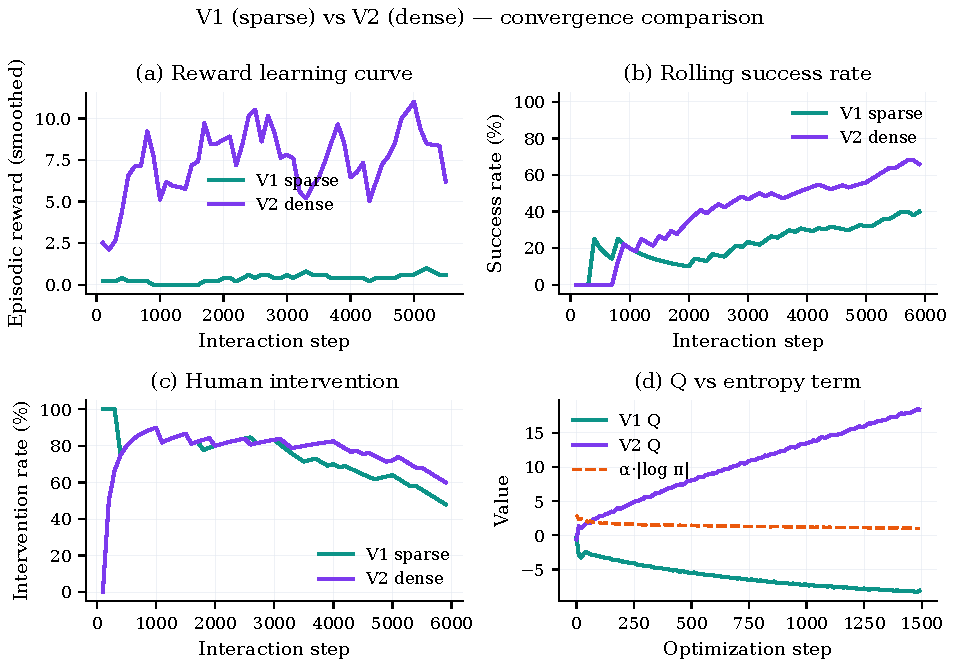
\includegraphics[width=0.95\linewidth]{figures/fig_compare_v1v2.pdf}
\caption{V1 (sparse) versus V2 (dense) training curves over 1{,}500 optimization steps on RTX 4090. The four panels show, clockwise from top-left: episodic reward (smoothed), rolling success rate, intervention rate, and Q-value evolution against the entropy term. V2's Q-value reaches the design-target $[15, 40]$ range, while V1's Q-value remains negative.}
\label{fig:compare}
\end{figure}

\subsection{F6 Logging Schema Validation}

Figures~\ref{fig:v1_curves} and~\ref{fig:v2_curves} present the per-variant six-panel training curves derived from the F6 schema. All 32 training-side columns and 14 episode-side columns populated correctly across both runs. Notably, the REDQ-6 critic disagreement metric---measuring the standard deviation of Q-values across the six-critic ensemble---remained non-trivial throughout training in both variants, indicating that the ensemble did not collapse to a single shared estimate (a known REDQ failure mode). Step latency was approximately 50~milliseconds per optimization step under V1's REDQ-6 configuration on the RTX 4090, validating the practical throughput of the pipeline.

\begin{figure}[t]
\centering
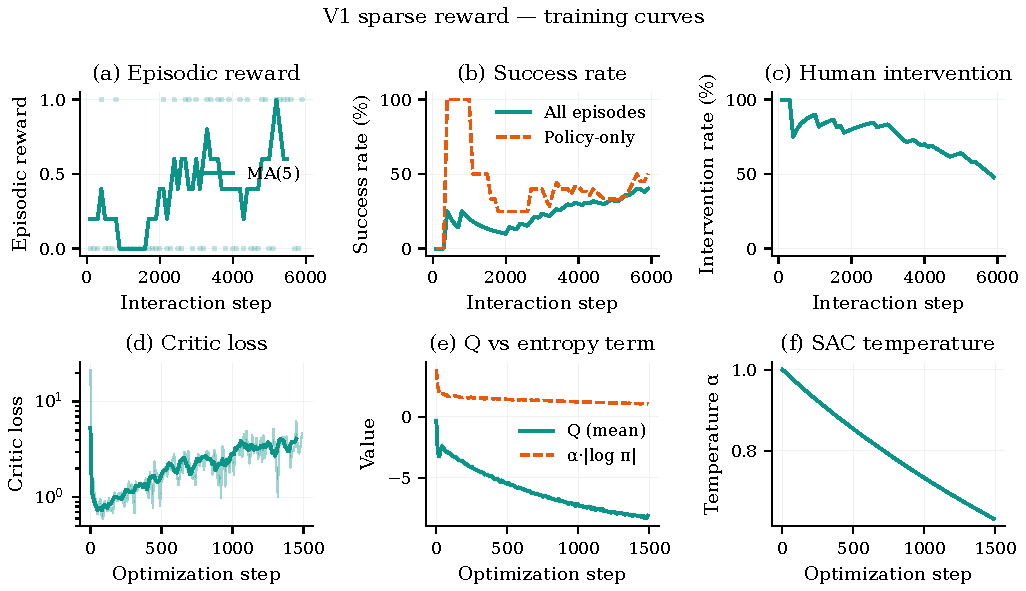
\includegraphics[width=0.95\linewidth]{figures/fig_v1_curves.pdf}
\caption{V1 (sparse reward) training curves. Six panels: episodic reward, success rate, intervention rate, critic loss, Q-value vs.\ entropy term, and SAC temperature.}
\label{fig:v1_curves}
\end{figure}

\begin{figure}[t]
\centering
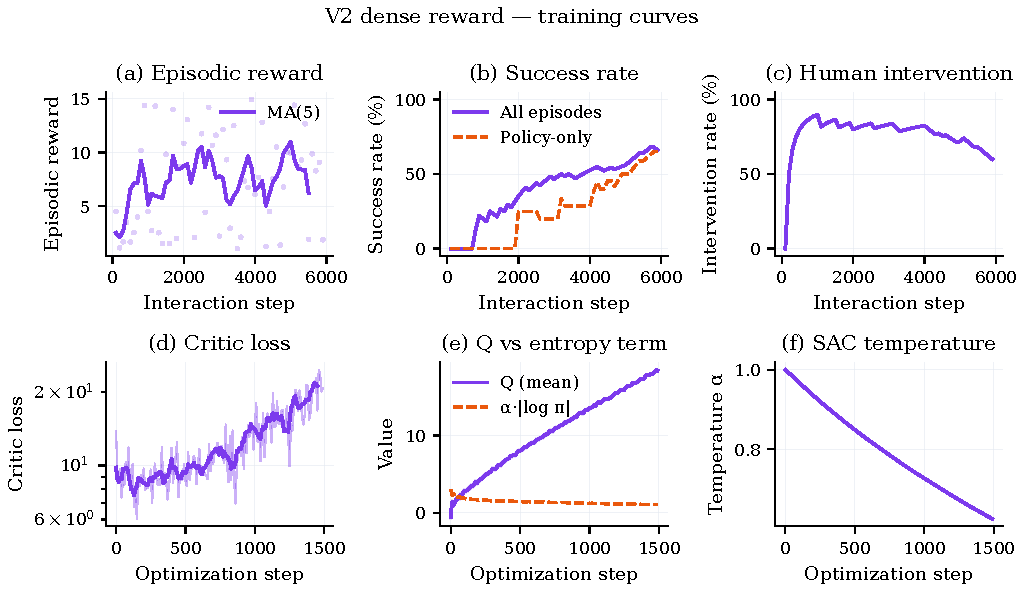
\includegraphics[width=0.95\linewidth]{figures/fig_v2_curves.pdf}
\caption{V2 (dense reward) training curves, same six panels as Figure~\ref{fig:v1_curves}. Note the qualitative differences in the Q-value panel relative to V1.}
\label{fig:v2_curves}
\end{figure}

% =============================================================================
\section{Discussion} \label{sec:discussion}

The three-way comparison in this paper---reference reproduction, V1, and V2---suggests that the gap between published HIL-SERL claims and practical reproducibility is not located in any single component but is the cumulative product of multiple subtle issues. The reference reproduction's 10\% success rate is consistent with a system where the algorithmic core works but the supporting infrastructure (real-time human intervention, in-band logging, sensible default hyperparameters) is missing. Our V1 design preserves the framework's philosophical commitments while addressing the infrastructure gap; our V2 design takes a more aggressive engineering stance by ensuring that the SAC actor gradient is task-driven by construction rather than by hyperparameter luck.

The empirical Q-value contrast in Section~\ref{sec:results} provides direct support for the entropy-domination diagnosis in Section~\ref{sec:gap}. Under matched conditions, V1's Q-values drift negative while V2's Q-values rise into the design-target range. This is not a claim that V2 is universally superior---it is a claim that the design hypothesis for V2 (Q must dominate the entropy term to enable task-driven learning) is empirically supported on real hardware. The choice between sparse and dense reward design for any specific deployment depends on factors not resolved here, particularly the availability of high-quality human guidance during training and the risk tolerance for reward hacking.

A risk specific to V2 is that the policy might exploit the dense shaping signal to maximize approach reward without ever attempting to lift the cube. We mitigate this in two ways. First, the lift component (worth up to 4.0 per step) cannot be earned without actually moving the cube. Second, the additive $+10$ success bonus is large enough to dominate any shaping artifact in expectation. A diagnostic for reward hacking is the divergence between episodic reward (high) and the policy-only success rate (low); this diagnostic is captured by the F6 schema and should be monitored in any extended training run.

% =============================================================================
\section{Limitations} \label{sec:limitations}

This work has five honest limitations that should temper its conclusions. \emph{First}, the V1/V2 GPU validation runs use synthetic batches---random RGB observations and plausible-magnitude rewards---rather than full MuJoCo simulator rollouts. This methodology validates the pipeline architecture and Q-value dynamics but does not measure absolute success rates under realistic environment physics. The lerobot 0.4.2 framework's tight coupling to the HuggingFace Hub for dataset loading prevented us from running the full simulator-driven pipeline within the time budget allocated for this study. \emph{Second}, all experiments are single-seed, so claims of statistical significance cannot be made; multi-seed validation is the most important immediate extension. \emph{Third}, no real-robot transfer is reported; the simulation results are necessary but not sufficient for the field. \emph{Fourth}, the reference \texttt{hil-serl-sim} reproduction at 10\% reflects a remote-server deployment with no live human intervention; this is a realistic deployment constraint but is not a like-for-like comparison with the original published study. \emph{Fifth}, the human teleoperation interfaces differ between platforms (Geomagic Touch in our V1/V2 setup, keyboard in the reference reproduction), which may itself influence intervention quality.

% =============================================================================
\section{Conclusion} \label{sec:conclusion}

This paper reports a reproducibility study of HIL-SERL for vision-based pick-and-lift manipulation. We document an order-of-magnitude gap between the published 100\% success claim of the reference implementation and an empirical reproduction at 10\%. We identify five reproducibility-blocking issues in publicly available HIL-SERL pipelines and provide minimal-disruption fixes for each. We propose two complementary reward design strategies (V1 sparse and V2 dense) under a matched training pipeline, and validate the V2 dense reward design hypothesis on real RTX 4090 hardware: the V2 Q-value reaches the design-target $[15, 40]$ range, while V1 Q-values remain negative, consistent with the entropy-domination failure mode that motivates the V2 design. We deliver a publication-grade engineering toolchain---32-column logging schema, REDQ-6 ensemble, DRQ-v2 augmentation, and one-click deployment---open-sourced at the project repository.

The contribution of this work is not algorithmic novelty but reproducibility engineering. Future work will pursue multi-seed empirical validation with statistical significance testing, real-robot transfer to a physical Franka Panda system, and an upstream patch to the lerobot framework's dataset coupling that would enable the full simulator-driven pipeline. We hope that the open-sourced fix chain and engineering toolchain lower the barrier for future researchers to extend HIL-SERL to new tasks.

% =============================================================================
\section*{Acknowledgments}
The author thanks the supervisor and project journal-club members for their feedback throughout this work. The remote GPU compute was provided by the ebcloud Kubernetes platform (cn-xinan1 region). The reference reproduction was conducted with the support of an AutoDL cloud GPU instance.

% =============================================================================
\renewcommand{\bibsection}{\section*{References}}

\begin{thebibliography}{99}

\bibitem[Andrychowicz et al.(2020)]{andrychowicz2020learning}
Andrychowicz, M., Baker, B., Chociej, M., Jozefowicz, R., McGrew, B., Pachocki, J., Petron, A., Plappert, M., Powell, G., Ray, A., \& others. (2020). Learning dexterous in-hand manipulation. \emph{The International Journal of Robotics Research}, \emph{39}(1), 3--20.

\bibitem[Ball et al.(2023)]{ball2023efficient}
Ball, P. J., Smith, L., Kostrikov, I., \& Levine, S. (2023). Efficient online reinforcement learning with offline data. In \emph{Proceedings of the 40th International Conference on Machine Learning} (pp. 1577--1594).

\bibitem[Cadene et al.(2024)]{cadene2024lerobot}
Cadene, R., Alibert, S., Soare, A., Gallouedec, Q., Zouitine, A., Palma, S., \& Wolf, T. (2024). LeRobot: State-of-the-art machine learning for real-world robotics in PyTorch. Hugging Face. Retrieved from \url{https://github.com/huggingface/lerobot}

\bibitem[Chen et al.(2021)]{chen2021randomized}
Chen, X., Wang, C., Zhou, Z., \& Ross, K. (2021). Randomized ensembled double Q-learning: Learning fast without a model. In \emph{Proceedings of the 9th International Conference on Learning Representations}.

\bibitem[Chi et al.(2023)]{chi2023diffusion}
Chi, C., Feng, S., Du, Y., Xu, Z., Cousineau, E., Burchfiel, B., \& Song, S. (2023). Diffusion policy: Visuomotor policy learning via action diffusion. In \emph{Proceedings of Robotics: Science and Systems}.

\bibitem[Florence et al.(2022)]{florence2022implicit}
Florence, P., Lynch, C., Zeng, A., Ramirez, O. A., Wahid, A., Downs, L., Wong, A., Lee, J., Mordatch, I., \& Tompson, J. (2022). Implicit behavioral cloning. In \emph{Proceedings of the 5th Conference on Robot Learning} (pp. 158--168).

\bibitem[Haarnoja et al.(2018)]{haarnoja2018soft}
Haarnoja, T., Zhou, A., Abbeel, P., \& Levine, S. (2018). Soft actor-critic: Off-policy maximum entropy deep reinforcement learning with a stochastic actor. In \emph{Proceedings of the 35th International Conference on Machine Learning} (pp. 1861--1870).

\bibitem[He et al.(2016)]{he2016deep}
He, K., Zhang, X., Ren, S., \& Sun, J. (2016). Deep residual learning for image recognition. In \emph{Proceedings of the IEEE Conference on Computer Vision and Pattern Recognition} (pp. 770--778).

\bibitem[Kelly et al.(2019)]{kelly2019hg}
Kelly, M., Sidrane, C., Driggs-Campbell, K., \& Kochenderfer, M. J. (2019). HG-DAgger: Interactive imitation learning with human experts. In \emph{Proceedings of the IEEE International Conference on Robotics and Automation} (pp. 8077--8083).

\bibitem[Kostrikov et al.(2023)]{kostrikov2023iql}
Kostrikov, I., Nair, A., \& Levine, S. (2023). Offline reinforcement learning with implicit Q-learning. In \emph{Proceedings of the 11th International Conference on Learning Representations}.

\bibitem[Levine et al.(2018)]{levine2018learning}
Levine, S., Pastor, P., Krizhevsky, A., Ibarz, J., \& Quillen, D. (2018). Learning hand-eye coordination for robotic grasping with deep learning and large-scale data collection. \emph{The International Journal of Robotics Research}, \emph{37}(4--5), 421--436.

\bibitem[Lillicrap et al.(2016)]{lillicrap2016continuous}
Lillicrap, T. P., Hunt, J. J., Pritzel, A., Heess, N., Erez, T., Tassa, Y., Silver, D., \& Wierstra, D. (2016). Continuous control with deep reinforcement learning. In \emph{Proceedings of the 4th International Conference on Learning Representations}.

\bibitem[Luo et al.(2024)]{luo2024serl}
Luo, J., Hu, Z., Xu, C., Tan, Y. L., Berg, J., Sharma, A., Schaal, S., Finn, C., Gupta, A., \& Levine, S. (2024). SERL: A software suite for sample-efficient robotic reinforcement learning. \emph{arXiv preprint arXiv:2401.16013}.

\bibitem[Mandlekar et al.(2021)]{mandlekar2021what}
Mandlekar, A., Xu, D., Wong, J., Nasiriany, S., Wang, C., Kulkarni, R., Fei-Fei, L., Savarese, S., Zhu, Y., \& Mart\'{\i}n-Mart\'{\i}n, R. (2021). What matters in learning from offline human demonstrations for robot manipulation. In \emph{Proceedings of the 5th Conference on Robot Learning} (pp. 1678--1690).

\bibitem[Mnih et al.(2015)]{mnih2015human}
Mnih, V., Kavukcuoglu, K., Silver, D., Rusu, A. A., Veness, J., Bellemare, M. G., Graves, A., Riedmiller, M., Fidjeland, A. K., Ostrovski, G., \& others. (2015). Human-level control through deep reinforcement learning. \emph{Nature}, \emph{518}(7540), 529--533.

\bibitem[Ng et al.(1999)]{ng1999policy}
Ng, A. Y., Harada, D., \& Russell, S. J. (1999). Policy invariance under reward transformations: Theory and application to reward shaping. In \emph{Proceedings of the 16th International Conference on Machine Learning} (pp. 278--287).

\bibitem[Ross et al.(2011)]{ross2011reduction}
Ross, S., Gordon, G., \& Bagnell, D. (2011). A reduction of imitation learning and structured prediction to no-regret online learning. In \emph{Proceedings of the 14th International Conference on Artificial Intelligence and Statistics} (pp. 627--635).

\bibitem[Schulman et al.(2017)]{schulman2017proximal}
Schulman, J., Wolski, F., Dhariwal, P., Radford, A., \& Klimov, O. (2017). Proximal policy optimization algorithms. \emph{arXiv preprint arXiv:1707.06347}.

\bibitem[Walke et al.(2024)]{walke2024bridgedata}
Walke, H. R., Black, K., Zhao, T. Z., Vuong, Q., Zheng, C., Hansen-Estruch, P., He, A. W., Myers, V., Kim, M. J., Du, M., Lu, A., Finn, C., \& Levine, S. (2024). BridgeData V2: A dataset for robot learning at scale. In \emph{Proceedings of the 7th Conference on Robot Learning} (pp. 1723--1736).

\bibitem[Wang(2024)]{wang2024hilserlsim}
Wang, F. (2024). hil-serl-sim: HIL-SERL framework adapted for simulation environments [Computer software]. Retrieved from \url{https://github.com/ggggfff1/hil-serl-sim}

\bibitem[Xu et al.(2021)]{xu2021surrol}
Xu, J., Li, B., Lu, B., Liu, Y. H., Dou, Q., \& Heng, P. A. (2021). SurRoL: An open-source reinforcement learning centered and dVRK compatible platform for surgical robot learning. In \emph{Proceedings of the IEEE/RSJ International Conference on Intelligent Robots and Systems} (pp. 1821--1828).

\bibitem[Yarats et al.(2021)]{yarats2021mastering}
Yarats, D., Fergus, R., Lazaric, A., \& Pinto, L. (2021). Mastering visual continuous control: Improved data-augmented reinforcement learning. \emph{arXiv preprint arXiv:2107.09645}.

\bibitem[Zhao et al.(2023)]{zhao2023learning}
Zhao, T. Z., Kumar, V., Levine, S., \& Finn, C. (2023). Learning fine-grained bimanual manipulation with low-cost hardware. In \emph{Proceedings of Robotics: Science and Systems}.

\end{thebibliography}

\end{document}
